\documentclass[10pt, a4paper]{article}

\usepackage[a4paper, total={7in, 10in}]{geometry}
\usepackage{lscape} 
\usepackage[latin1]{inputenc}
\usepackage{palatino}
\usepackage{color}
\usepackage{lipsum}
\usepackage{rotating}
\usepackage{tabularx}
\usepackage{hyperref}
\usepackage{biblatex}
\addbibresource{sample.bib}

%% a point to check
\definecolor{checkcolor}{rgb}{0.75, 0.75, 0.75}
\newsavebox{\definitionbox}
\newenvironment{checkit}{%
\begin{lrbox}{\definitionbox}
\begin{minipage}[t]{0.95\textwidth}%
}%
{\end{minipage}
\end{lrbox}%
\begin{center}{\colorbox{checkcolor}{\usebox{\definitionbox}}}%
\end{center}}

\title{Software Engineering \\ Synopsis \\ Run (Android Application)}
\author{Dhruv Kudale and Vatsal Unadkat}
\date{January 2019}


\begin{document}
\maketitle

\begin{abstract}
Running is a very common sport among millions of people. It's an effective form of exercise but due to the lack of motivation a lot of people struggle to start running. Thereby the purpose of the android application would be to help them to look forward to start running whether it is their first time or trying to develop or maintain it as a habit. It also focuses to keep them engaged and focus on improving their pace time.

\end{abstract}

\section{Introduction}
The Run android application would be to help runners to look forward to start running whether it is their first time or trying to develop/maintain it as a habit. It also focuses to keep them engaged and focus on improving their pace time. The application will benefit runners and lazy runners in improving their pace. The application will adjust the music according to the BPM value of the runner. The application will enhance everyday running activity and also give an enhanced running experience. This will in turn motivate reluctant runners to run and have a better performance.\\ The purpose of this Synopsis document is to provide a detailed overview of our android application Run, its objectives, goals and methodology with the aid of research paper analysis.The research papers are studied for understanding their mode of approach, aspects that can be advantageous and/or disadvantageous to the project and their respective accuracies. 


\section{Literature Review}

The tabular literature review comprising of analysis of relevant journal research papers is displayed below in table 1.1. The comparative study consists of 15 research papers related to the topics of pedometer accuracy and music prediction with their advantages, disadvantages  and particular accuracy.Many researches are done in the past decades related to smartphone pedometer accuracy, music prediction algorithms, tags research, psychological effects of music on running, etc in the journals published in the field of statistics, smartphones, devices, sensors, physical fitness, sports and exercise, music, psychology, etc. The document is written with an intention to understand the existing backbone research made in the interest of the application.Following papers were read, ananlyzed and tabulated as follows
\cite{1}Accuracy of a smartphone pedometer application,   
\cite{2}Pedometers to promote physical activity,  
\cite{4}Music auto-tagging using deep Recurrent Neural Networks, 
\cite{5}Tag-Aware Dynamic Music Recommendation, 
\cite{6}Humans are able to self-paced constant running accelerations, 
\cite{7}Comparison of Several Algorithms to Estimate Activity Counts, 
\cite{8}Pedometer-Measured Physical Activity, 
\cite{9}Effects of synchronous music on treadmill running among elite triathletes, 
\cite{10}The effect of music type on running perseverance and coping with effort sensations, 
\cite{11}A novel method for personalized music recommendation,  
\cite{12}How Accurate are Pedometer Cell Phone Applications, 
\cite{13}Expert Systems with Applications and 
\cite{14}Influence of non-level walking on pedometer accuracy
The row number of the following table corresponds to the research paper referred (See References).


\begin{landscape}
\begin{center}
Table 1.1
\bigbreak
\begin{tabular}{ | m{0.5cm} | m{3.5cm}| m{5cm} | m{4.5cm}| m{5cm}| m{5.5cm}|} 
\hline \hline
No. & Author and Year & Approach Used & Advantages & Disadvantages & Accuracy\\ 
\hline
\hline
1 & Bastien Presset, Balazs Laurenczy, Davide Malatesta in 2017 &18 People were tested with pedometers at arm,belt,etc at various speeds and tasks were performed & Study of smartphone pedometer and physical one showed that the former is either equally accurate or more accurate than the latter & Older devices, iphone and android devices were not tested at all; target group did not cover all cases & Smartphone pedometers are more accurate(2-6 kmph) and equally accurate above 6 kmph to physical pedometers\\ 
\hline
2 & David R. Lubans a, Philip J. Morgan, Catrine Tudor-Locke in 2009 & Systematic search of 6 electronic databases like physical activities, walking, etc against predetermined criteria was done & Target group and cases are similar to the project needs and hence helped to set goal settings & The approach used was a short term study so doesn't guarantee sustainability & Pedometers have been used successfully to to promote activity among youth\\ 
\hline
3 & Wonil Park, Victor J. Lee, Byungmo Ku, Hirofumi Tanaka in 2013-14 & Newer pedometers vs older ones placed at different positions were tested compared with hand tally counter  & Study was performed on a larger age group and various positions & Test duration was less and was carried on a treadmill which enforced participants to run continuously & Newer pedometers are more accurate than older ones for moderate speeds only but not for very slow and very fast speeds\\ 
\hline
4 & Guangxiao Song, Zhijie Wang, Fang Han, Shenyi Ding, Muhammad Ather Iqbal in 2017-18 & 2 stages of preprocessing of tags and ML by 5 layer recurrent neural networks & Various models enabling faster training speeds and lesser memory usage were used and evaluated & Tagging is inaccurate when duration is small. Model can take too long due to exploring gradiation or vanishing gradients & Accuracy increases with increase in the number of layers. 5 layer RNN was more accurate than that of 4 layer one\\ 
\hline
5 & Ervine Zheng, Gustavo Yukio Kondo, Stephen Zilora, Qi Yu in 2017-18 & The framework uses a Gaussian state-space model to capture preferences over time, which is used in music recommendation & Compression is done using LCPA and hence sparsity is taken care of & Collaborative filtering algorithms may fail recommend accurately a small portion of the user action is seen & A Gaussian state-space model is developed to determine evolution of preferences of users, making the overall recommendation time-sensitive and hence more accurate.\\ 
\hline
6 & Veronique Billat, Nicolas Brunel, Thomas Carbillet, Adeline Samson, 2018 & 5 people were made to run in random order for 3 exhaustive self paced accelerations trials and a descriptive model was chosen for further analysis & Recreational runners can maintain and apply distinct accelerations which is fruitful considering self paced targets & Middle aged runners were chosen for the study. The set was also small which did not consist of younger individuals & Runners are able to control and maintain subjective accelerations until exhaustion for about 1 min 36s to 20 min \\ 
\hline
7 &  V.H.Rodriguez, C.Medrano, I.Plaza, C.Corella, A.Abarca, J.A.Julian in 2018 & Carrying out comparison of four algorithms so that smartphone can produce results obtained with devices like GT3X+ & Smartphones can thus efficiently track physical activity that refers to self tracking, awareness an performance improvement & Walking and running speeds were 'self selected' and the test was performed only once & Algorithm 4 of measuring direct area under accelerometer curve gave the highest accuracy (minimum RMSE) \\ 
\hline
8 & Michael W. Beets, Daniel Bornstein, Aaron Beighle,
Bradley J. Cardinal, Charles F. Morgan in 2010 & Comparison and exploring the physical activity patterns of young users via pedometers from around 13 countries & Data set is large, spanning a lot of regions of the world composed of students from ages 11 to 18 which is part of the target group intended & Variations in data collection procedure in different places may account for differences in observed steps per day & Pedometers with a standard metric are one of the few valid, reliable and accurate measures of youth physical activity \\ 
\hline
\end{tabular}
\end{center}

\end{landscape}

\begin{landscape}
\begin{center}
Table 1.1
\bigbreak
\begin{tabular}{ | m{0.5cm} | m{3.5cm}| m{5cm} | m{4.5cm}| m{5cm}| m{5.5cm}|} 
\hline \hline
No. & Author and Year & Approach Used & Advantages & Disadvantages & Accuracy\\ 
\hline
\hline
9 & Peter C. Terry, Costas I. Karageorghis, Alessandra Mecozzi Saha, Shaun DAuria in 2011 & 11 runners were made to run on a treadmill with music and once without music to evaluate time to exhaustion, mood response, oxygen consumption, RPE, etc & Proves that music can provide ergogenic and psychological benefits during physical activity which motivate runners & Young recreational runners or beginners were not considered in the study & Music presence benefits by increasing mood responses, time to exhaustion by 18.1 to 19.7 percent and reduces RPE \\ 
\hline
10 & G. Tenenbaum, R. Lidor, N. Lavyan, K. Morrow, S. Tonnel, A. Gershgoren, J. Meis in 2001-02 & Participants ran on treadmill and hilly terrain four times in a setting of music(Rock, Inspirational and Dance) and without music  to compare RPE, HR, etc & Participants were beginners to moderate runners between ages 18 to 34 (part of target group) and hilly terrain was also considered & Heavy physical exertion was used which is not practically observed; wrong type of music failed to influence RPE & Right type (inspirational) music can benefit running as 63 percent participants felt motivated during many phases of the run \\ 
\hline
11 & Cheng-Che Lu and Vincent S. Tseng in 2009 & Combines the content-based, collaboration-based and emotion-based methods & Constructed a system that can recommend the music to users after mining logs of user on music listening records & 
Fails to avoid repeatedly recommending the "disfavoured music" for users and does not  recommend more interesting music for users besides the ones users have been used to listen & Users may be not interested in highly rated music and cannot recommend the music which is not rated by anyone\\ 
\hline
12 & Anna Akerberg, Maria Linden, and Mia Folke in 2012 & 10 test people using six different free pedometer applications for three different cell phones were tested &  Only specific combinations showed a good accuracy with reasonable low standard deviation & Being an old research paper so the technology might be outdated that is the phone or its applications & The majority of applications evaluated in this study, did not show high accuracy\\ 
\hline
13 & Vanda Ho a , Rebecca K. Simmons b and Charlotte L. Ridgway in 2013 & Measure physical activity among adolescents independent of other behaviour change & Covered a wide range of adolescents (892) & Covered over a short time period (4 days) and the study was also more focused on the changes that were gender specific & A lot of factors were taken into consideration such as age, gender, height, weight, BMI, body fat, etc which enhanced the accuracy of the results\\ 
\hline
14 & Anthony S. Leicht and Robert G. Crowther in 2009 & As most research papers on pedometers are conducted on flat surfaces this one is conducted on inclines and its effects on them & Wide variety for test subjects were used and consistency was maintained throughout the tests & Only 1 specific pedometer was used for the study accompanied by short test durations and overestimation during going down staircases in some cases & Exhibited good accuracy during incline walking up to 10 percent \\ 
\hline
\end{tabular}
\end{center}

\end{landscape}

Few aspects encountered while reviewing literature are analyzed in the research gaps.

\section{Research Gaps}
A considerable amount of research is done in running, smart phone pedometers, ways of music prediction as well as effects of music on running. Following points mention the narrow domains of which limited, insufficient research is made which eventually restricts the ability to answer or conclude aspects related to the matter. 
\begin{itemize}
\item Pedometer research in Android (particular) applications
\item Habit of repeated recommendation for users apart from the ones users have been used to listen or for that of a segment of smaller duration
\item Verification of the accuracy from an external source with respect to music prediction 
\item Inclusion of young individuals with spontaneous and free running tests who are currently occupied in sedentary lifestyle or exercise less than thrice a week
\end{itemize}

\section{Objectives}

The main objective of this project is to build an effective and beneficial music recommendation system and a reliable pedometer keeping in mind the young individuals, their needs, way of approach and sedentary lifestyle. The aim is to induce positive atmosphere that will motivate beginners as well as runners with decent stamina to improve and maintain the habit of this basic physical activity.Following are one of 
the main objectives 
\begin{itemize}
\item To predict and deliver the most suitable track for the runner in the ongoing phase of the run so as to keep the runner engaged in the process.The assumption can be made that exercising to fast tempo music or that appropriately suggested music should produce faster running performance.
\item To make a reliable pedometer that displays relevant, tactful and accurate pace reading and other statistics that will broadly enhance the mind of the runner during the run
\item To enable consideration of calendar events or festivals for favourable recommendation for the users 
\end{itemize}



\section{Methodology}

\begin{figure}[ht]
\begin{center}
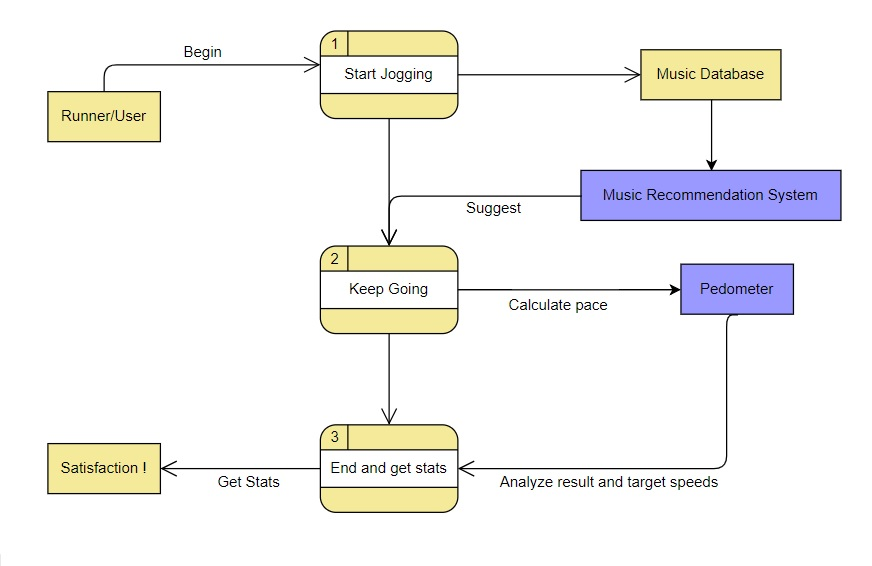
\includegraphics[scale=0.7]{./dataflow.jpg}
\end{center}
\caption{Schematic view of the application}
\label{Fig 1}
\end{figure}
The music recommendation system and the reliable pedometer are one of the major highlights of this project. Following figure shows a schematic analysis of the application with the user or runner point of view.\\
User will start running and during various phases of running the music recommendation system will suggest suitable track of dynamic duration based on the BPM value of the runner in order to improve the performance.For acheiving this, (although not a compulsory requirement) a database of the past runs with split timings per kilometre could help the application for its music predictions. The personal play-list of the user would also be of good help which can be added to the music database. \\
The pedometer will keep into account the required statistical information pertaining to the phase, real time improvement and changes occurring in the pace, target speed analysis,etc. Thus in the above mentioned manner, user can satisfactorily analyze his/her personal results, goal settings, etc and thereby improve the performance 

\section{Conclusion}
In this project, the aim is to develop an application that will motivate the runners to perform better.Android platform is used to implement this application. Every person nowadays posseses an android cell phone hence the reason. The application aims to induce some beneficial physical activity motivation (here in running) accompanied with proper, spontaneous and encouraging music suggestions which will direct in expanding the sedentary life of various young individuals.

\begin{thebibliography}{9} 

\bibitem{1} Accuracy of a smartphone pedometer application \\\texttt{https://www.sciencedirect.com/science/article/pii/S1728869X17303167}

\bibitem{2} Pedometers to promote physical activity
\\\texttt{https://www.sciencedirect.com/science/article/pii/S009174350900111X}, a study of electronic databases

\bibitem{3}Effect of walking speed in determining pedometer accuracy \\\texttt{https://www.sciencedirect.com/science/article/pii/S1728869X14000057}

\bibitem{4}Music auto-tagging using deep Recurrent Neural Networks
\\\texttt{https://www.sciencedirect.com/science/article/pii/S0925231218302431}, a process of recommendation

\bibitem{5}Tag-Aware Dynamic Music Recommendation
\\\texttt{https://www.sciencedirect.com/science/article/pii/S0957417418302446},using linear algebraic approach like matrix factorization, dimension reduction,etc

\bibitem{6}Humans are able to self-paced constant running accelerations
\\\texttt{https://www.sciencedirect.com/science/article/pii/S0378437118304941}, claiming that constant accelerations are obtained by the application of brief corrections

\bibitem{7}Comparison of Several Algorithms to Estimate Activity Counts
\\\texttt{https://www.sciencedirect.com/science/article/abs/pii/S1959031818300046}, four algorithms to get GT3X+ activity counts from accelerometer signals are compared.


\bibitem{8}Pedometer-Measured Physical Activity
\\\texttt{https://www.sciencedirect.com/science/article/pii/S0749379709007727}, physical activity level study among young people aged 5 to 18 years

\bibitem{9}Effects of synchronous music on treadmill running among elite triathletes
\\\texttt{https://www.sciencedirect.com/science/article/pii/S1440244011001186}

\bibitem{10}The effect of music type on running perseverance and coping with effort sensations 
\\\texttt{https://www.sciencedirect.com/science/article/pii/S1469029202000419}, examining the effect of music type on running time 

\bibitem{11}A novel method for personalized music recommendation
\\\texttt{https://www.sciencedirect.com/science/article/pii/S0957417409000591}, recommendation of the favored music from large amounts of digital music

\bibitem{12}How Accurate are Pedometer Cell Phone Applications 
\\\texttt{https://www.sciencedirect.com/science/article/pii/S221201731200518X}

\bibitem{13}Expert Systems with Applications 
\\\texttt{https://www.sciencedirect.com/science/article/pii/S0091743513000285},confirming whether wearing a pedometer associated with higher physical activity among adolescents

\bibitem{14}Influence of non-level walking on pedometer accuracy
\\\texttt{https://www.sciencedirect.com/science/article/pii/S144024400800008X}, accuracy of pedometer during non-level walking activities 


\end{thebibliography}

\printbibliography

\end{document}
